\documentclass[10pt, landscape]{article}
\usepackage[scaled=0.92]{helvet}
\usepackage{calc}
\usepackage{multicol}
\usepackage{ifthen}
\usepackage[a4paper,margin=5mm,landscape]{geometry}
\usepackage{amsmath,amsthm,amsfonts,amssymb}
\usepackage{color,graphicx,overpic}
\usepackage{hyperref}
\usepackage{newtxtext} 
\usepackage{enumitem}
\usepackage{amssymb}
\usepackage[table]{xcolor}
\usepackage{vwcol}
\usepackage{tikz}
\usetikzlibrary{arrows.meta}
\usetikzlibrary{calc}
\usepackage{mathtools}
\usepackage{nicematrix}
\usepackage[T1]{fontenc} %%% <--- NOTE THIS
% for relations
\usepackage{cancel}
\usepackage{ mathrsfs }
\usepackage{listings}
\usepackage{background}
\setlist{nosep}

\usepackage{etoolbox}
\makeatletter
\preto{\@verbatim}{\topsep=0pt \partopsep=0pt }
\makeatother

\backgroundsetup{
scale=1,
color=black,
opacity=0.2,
angle=0,
contents={%
  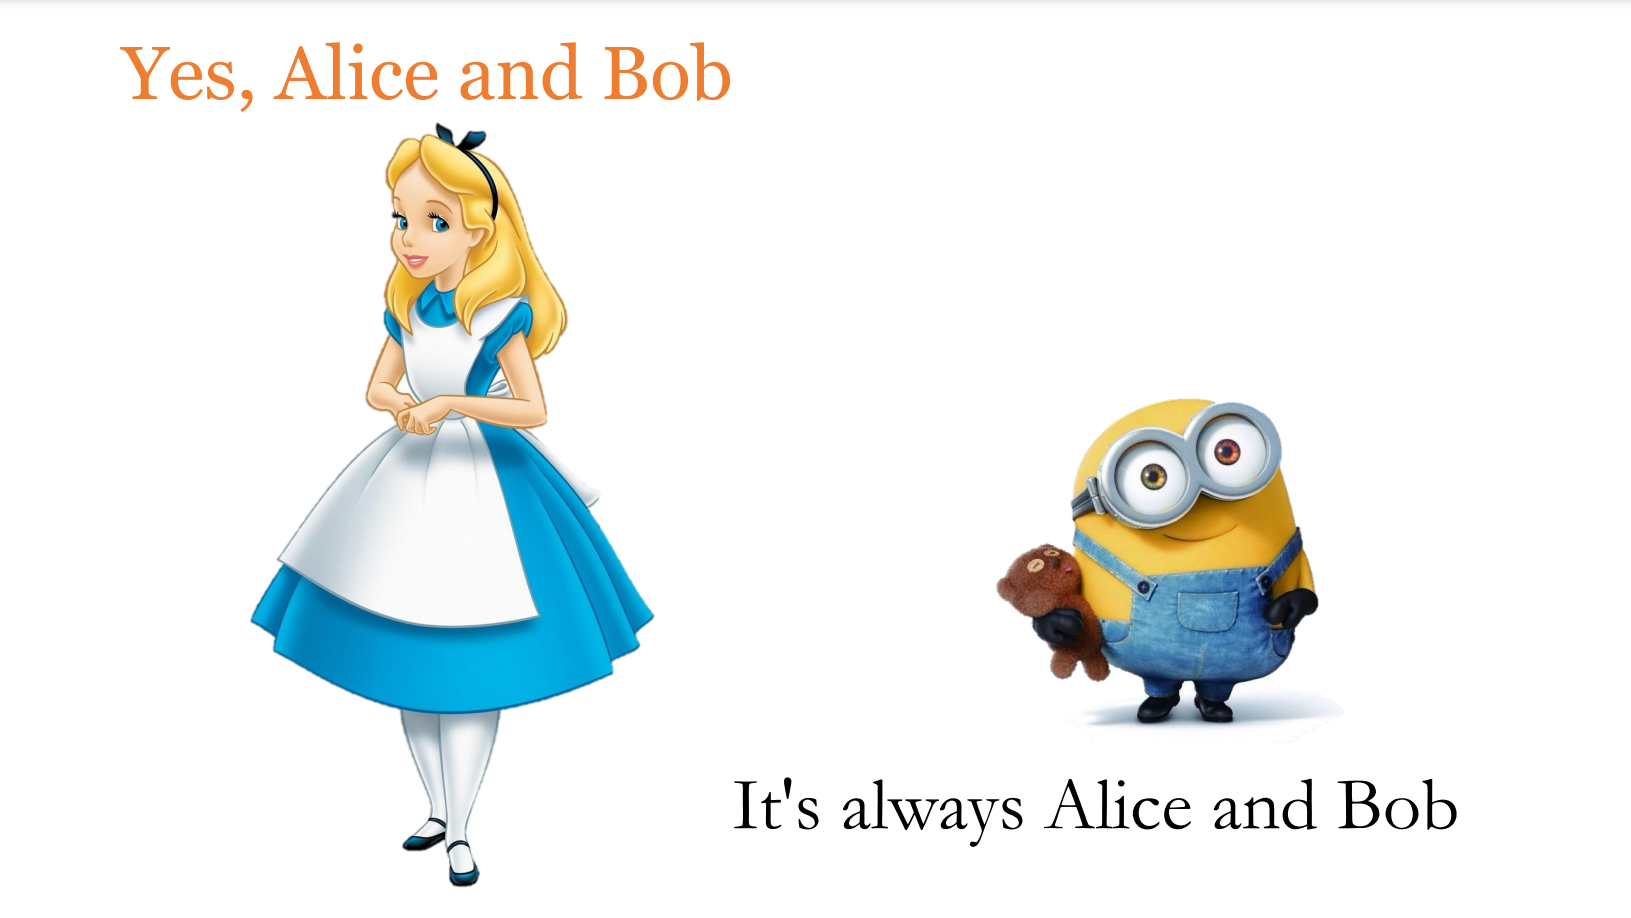
\includegraphics[width=\paperwidth,height=\paperheight]{alice.png}
  }%
}

\pdfinfo{
  /Title (CS2105.pdf)
  /Creator (TeX)
  /Producer (pdfTeX 1.40.0)
  /Author (Seamus)
  /Subject (Example)
  /Keywords (pdflatex, latex,pdftex,tex)}

\lstset{language=Java,keywordstyle={\bfseries \color{black}}}

% Turn off header and footer
\pagestyle{empty}

\newenvironment{tightcenter}{%
  \setlength\topsep{0pt}
  \setlength\parskip{0pt}
  \begin{center}
}{%
  \end{center}
}

% redefine section commands to use less space
\makeatletter
\renewcommand{\section}{\@startsection{section}{1}{0mm}%
                                {-1ex plus -.5ex minus -.2ex}%
                                {0.5ex plus .2ex}%x
                                {\normalfont\large\bfseries}}
\renewcommand{\section}{\@startsection{section}{2}{0mm}%
                                {-1explus -.5ex minus -.2ex}%
                                {0.5ex plus .2ex}%
                                {\normalfont\normalsize\bfseries}}
\renewcommand{\subsection}{\@startsection{subsection}{3}{0mm}%
                                {-1ex plus -.5ex minus -.2ex}%
                                {1ex plus .2ex}%
                                {\normalfont\small\bfseries}}%
\renewcommand{\familydefault}{\sfdefault}
\renewcommand\rmdefault{\sfdefault}
% makes nested numbering (e.g. 1.1.1, 1.1.2, etc)
\renewcommand{\labelenumii}{\theenumii}
\renewcommand{\theenumii}{\theenumi.\arabic{enumii}.}
\renewcommand\labelitemii{•}
%  for logical not operator
\renewcommand{\lnot}{\mathord{\sim}}
\renewcommand{\bf}[1]{\textbf{#1}}
\newcommand{\abs}[1]{\vert #1 \vert}
\newcommand{\Mod}[1]{\ \mathrm{mod}\ #1}

\makeatother
\definecolor{myblue}{cmyk}{1,.72,0,.38}
\everymath\expandafter{\the\everymath \color{myblue}}
% Define BibTeX command
\def\BibTeX{{\rm B\kern-.05em{\sc i\kern-.025em b}\kern-.08em
    T\kern-.1667em\lower.7ex\hbox{E}\kern-.125emX}}
\let\iff\leftrightarrow
\let\Iff\Leftrightarrow
\let\then\rightarrow
\let\Then\Rightarrow

% Don't print section numbers
\setcounter{secnumdepth}{0}

\setlength{\parindent}{0pt}
\setlength{\parskip}{0pt plus 0.5ex}
%% this changes all items (enumerate and itemize)
\setlength{\leftmargini}{0.5cm}
\setlength{\leftmarginii}{0.5cm}
\setlist[itemize,1]{leftmargin=2mm,labelindent=1mm,labelsep=1mm}
\setlist[itemize,2]{leftmargin=4mm,labelindent=1mm,labelsep=1mm}

%My Environments
\newtheorem{example}[section]{Example}
% -----------------------------------------------------------------------

\begin{document}
\raggedright
\footnotesize
\begin{multicols*}{3}

% multicol parameters
% These lengths are set only within the two main columns
\setlength{\columnseprule}{0.25pt}
\setlength{\premulticols}{1pt}
\setlength{\postmulticols}{1pt}
\setlength{\multicolsep}{1pt}
\setlength{\columnsep}{2pt}

\begin{center}
    \fbox{%
        \parbox{0.8\linewidth}{\centering \textcolor{black}{
            {\Large\textbf{CS2105}}
            \\ \normalsize{AY24/25 Sem 2}}
            \\ {\footnotesize \textcolor{myblue}{by ngmh}} 
        }%
    }
\end{center}

\section{Internet}
\begin{itemize}
    \item Network of connected computing devices
    \item Internet is NOT World Wide Web
    \item World Wide Web is one of the services that runs over the Internet
\end{itemize}

\subsection{Network Edge}
\begin{itemize}
    \item Consists of end hosts, servers, etc.
    \item Hosts run network applications
    \item Applications communicate using protocols, which define format and order of messages as well as actions to take
    \item Hosts access the internet through access networks e.g. Residential, Institutional, Mobile
    \item Wireless Access Network: Connects hosts to router via base station / access point
    \begin{itemize}
        \item Wireless LANs: Wi-Fi, Within building
        \item Wide-area wireless access: 3G, 4G, Provided by telco (cellular) operator
    \end{itemize}
    \item Physical Media: How hosts connect to access network
    \begin{itemize}
        \item Guided: Solid media, e.g. Fiber
        \item Unguided: Free propagation, e.g. Wi-Fi, cellular
    \end{itemize}
\end{itemize}

\subsection{Network Core}
\begin{itemize}
    \item Consists of ISPs, routers, etc.
    \item Mesh of interconnected routers
    \item Circuit Switching
    \begin{itemize}
        \item Resources allocated and reserved for transmission
        \item Setup required, but guaranteed performance
        \item Circuit segment is idle if not used by call (no sharing)
        \item Common in traditional telephone networks
        \item Divide bandwidth into pieces by frequency and time
    \end{itemize}
    \item Packet Switching (e.g. The Internet)
    \begin{itemize}
        \item Host breaks message down into packets of length $L$ and transmits on a link with transmission rate $R$ (a.k.a bandwidth)
        \item Packet transmission delay $=L/R$
        \item Packets are passed along from one router to the next across links
        \item Store and Forward: Entire packet must arrive at a router before being transmitted out
        \item Routing and Addressing: Routers determine route taken by packets, which need to carry source and destination information
        \item No setup needed, but resources are shared and transmission is best effort
    \end{itemize}
    \item Connecting ISPs to each other is costly, so there are regional and global ISPs which act as middlemen
    \item Peering Link: Between 2 ISPs
    \item Internet Exchange Point: Middleman between 2 ISPs
    \item Content providers might also run their own network
    \item Authorities
    \begin{itemize}
        \item IP Address and Internet Naming administered by Network Information Centre (NIC)
        \item The Internet Society (ISOC): Leadership in Internet related standards
        \item The Internet Architecture Board (IAB): Authority to issue and update technical standards regarding Internet protocols
        \item Internet Engineering Task Force (IETF): Protocol engineering, development, and standardisation
    \end{itemize}
\end{itemize}

\subsection{Delay and Loss}
\begin{itemize}
    \item Packets queue in router buffers to be sent out
    \item When capacity is reached, arriving packet will be dropped and lost
    \item Lost packet may be retransmitted by previous node or source or not at all
    \item Processing Delay: Time to check bit errors, and determine output link
    \item Queueing Delay: Time waiting in queue for transmission, depends on congestion level
    \item Transmission Delay: $L/R$, time taken for packet to be fully sent out
    \item Propagation Delay: $d/s$, time taken for packet to travel across link
    \item These 4 factors form end-to-end packet delay
    \item Throughput: How many bits can be transmitted per unit time
    \item Link Capacity / Bandwidth is measured for a specific link
    \item Units: 1 byte = 8 bits, Micro, Milli, Standard, Kilo, Mega, Giga, Tera
    \item Capital B = bytes, Small B = bits
\end{itemize}

\subsection{Protocol Layers}
\begin{itemize}
    \item Modularise large and complex systems
    \item Each layer servers their own purpose, with simple interfaces between them
    \item Layers:
    \begin{itemize}
        \item Application: Treat Internet as a black box
        \item Transport: Process-to-process data transfer
        \item Network: Routing of datagrams from host to host
        \item Link: Data transfer between neighbouring network elements
        \item Physical: Bits on the wire / air
    \end{itemize}
\end{itemize}

\section{Application Layer}
\subsection{Architecture}
\begin{itemize}
    \item Client-Server Architecture
    \begin{itemize}
        \item Server waits for incoming requests and provides requested service to client
        \item Client initiates contact with server and requests service from it
    \end{itemize}
    \item P2P Architecture
    \begin{itemize}
        \item No always on server, end systems directly communicate
        \item Peers request and provide service to other peers
        \item Highly scalable, but difficult to manage
    \end{itemize}
    \item Hybrid of both with centralised server and P2P, e.g.  isntant messaging
\end{itemize}

\subsection{Service Criteria}
\begin{itemize}
    \item Data Integrity: Whether they need reliable data transfer (e.g. file transfer) or can they tolerate data loss (e.g. audio streaming)
    \item Throughput: How much bandwidth does the app need (e.g. multimedia)
    \item Timing: Some apps require low delay to be effective (e.g. online games)
    \item Security: Encryption and data integrity
\end{itemize}

\subsection{Protocols}
\begin{itemize}
    \item They define:
    \begin{itemize}
        \item Types of messages exchanged
        \item Rules for when to send and respond messages
        \item Message Syntax: What fields are in messages and how are they delimited
        \item Message Semantics: Meaning of information in fields
    \end{itemize}
    \item Open protocols: Defined in RFCs and allow for interoperability
    \item Proprietary: Privatized and not released to public
    \item Identifying Network Processes:
    \begin{itemize}
        \item IP Address (Globally Unique): Identifies Host, IPv4 has 32 bits split into 4 bytes in dotted decimal notation, v6 has 128 bits split into 8 sets of 2 bytes in hexadecimal notation
        \item Port Number (Locally Unique): 16 bit number, 1 to 1023 are reserved
        \item Port numbers are assigned by IANA
    \end{itemize}
    \item User Datagram Protcol and Transmission Control Protocol
\end{itemize}

\subsection{The Web}
\begin{itemize}
    \item WWW Consortium: Global Open standards
    \begin{itemize}
        \item HyperText Markup Language (HTML): Explains how it should be interpreted
        \item Uniform Resource Locator (URL): Explains how to locate resources
        \item HyperText Transfer Protocol (HTTP): Explains how to access those resources
    \end{itemize}
    \item Webpage: Base HTML file and other referenced objects (which each have their own URL)
    \item Resource are requested using HTTP which uses a client / server model
\end{itemize}

\subsection{HTTP}
\begin{itemize}
    \item Uses TCP as a transport service
    \item Round-Trip Time (RTT): Time taken for a packet to travel from client to server and back
    \item HTTP/1.0: New connection is established for every resource requested, time taken is $2RTT+$ transmission time
    \item HTTP/1.1 Pipelining: New request is made before receiving response of old requests, as soon as a referenced object is encountered
    \item Persistent HTTP: Server leaves connection open after sending response, connection is reused, can be as little as one RTT
    \item HTTP/2 Multiplexing: Response can come back in any order, even partially
    \item Request:
\begin{verbatim}
    GET /~cs2105/demo.html HTTP/1.1\r\n
    Host: www.comp.nus.edu.sg\r\n
    User-Agent: Mozilla/5.0\r\n
    Connection: close\r\n
\end{verbatim}
    \item Response:
\begin{verbatim}
    HTTP/1.1 200 OK\r\n
    Date: Wed, 01 Jul 201508:47:52 GMT\r\n
    Connection: Keep-Alive\r\n
    Content-Length: 73\r\n
    Content-Type: text/html\r\n
    Keep-Alive: timeout=5, max=100\r\n
    \r\n
    <!DOCTYPE html>...
\end{verbatim}
    \item Status Codes: 200 Ok, 301 Moved Permanently, 304 Not Modified, 403 Forbidden, 404 Not Found, 500 Internal Server Error
    \item Uses Cookies to keep track of state, server does not store info about connection
    \item Caching: Don't send object if client has up-to-date version of resource
    \item Use Conditional Get to determine, with If-modified-since: <date> header in request, which might get a 304 response with no object if up-to-date
\end{itemize}

\subsection{DNS}
\begin{itemize}
    \item Domain Name System
    \item Translate between hostname and IP address
    \item Stored as Resource Records with different types (A = address, NS = nameserver, CNAME = canonical name, MX = mail exchange) and TTL
    \item Stored in distributed hierarchical Databases
    \item 13 Root name servers worldwide
    \item Top Level domain servers for each domain suffix
    \item Authoritative servers: DNS Servers belonging to organisations, provides authoritative hostname to IP mappings for organisation's named hosts
    \item Local DNS Server: Does not strictly belong to hierarchy, each ISP has one
    \item Recursive Query: Query is forwarded upwards until it is found
    \item Iterative Query: Query is made separately to each level up of the chain from local DNS server
    \item DNS Caching: Mapping is cached once name server learns about it
\end{itemize}

\section{Socket Programming}
\begin{itemize}
    \item A host runs several processes: Top level execution containers with independent memory space
    \item Each process can have multiple threads which share the same memory
    \item Processes in the same host communicate with inter-process communication defined by OS while those in different hosts communicate by exchanging messages according to protocols
    \item Processes are identified by IP Address + Port Number
\end{itemize}

\subsection{Sockets}
\begin{itemize}
    \item Sockets are the abstraction interface between processes and transport layer protocols
    \item Stream Socket uses TCP, while Datagram Socket uses UDP
    \item UDP Socket:
    \begin{itemize}
        \item Only one socket is needed, communications is shared
        \item Application creates packet with recipient, OS attaches return info
        \item Receiver identifies sender by extracting address information
    \end{itemize}
    \item TCP Socket:
    \begin{itemize}
        \item Data flows in a continuous stream
        \item Connection established between 2 processes
        \item Server listens on socket and forks a new one when contacted by client, distinguishing by client address info
        \item Client creates socket to establish a connection with server
        \item Every connection has its own socket instance
    \end{itemize}
\end{itemize}

\section{Reliable Protocols}
\begin{itemize}
    \item Transport layer provides process-to-process communication
    \item Network layer provides host-to-host, best-effort and unreliable communication
    \item Unreliable channel might corrupt / drop / re-order / delay packets
    \item RDT: Reliable Delivery Transfer
    \item Finite State Machine: Describe sender and receiver of a protocol
    \item rdt1.0: Reliable channel
    \item rdt2.0: Channel with bit errors
    
    Use checksum to detect, requires ACK / NAK and retransmissions, but this could be fatal if ACK is corrupted
    \item rdt2.1: Add sequence number to handle duplicates, retransmits if ACK / NAK is garbled
    \item rdt2.2: Replace NAK with ACK of last correctly received packet
    \item rdt3.0: May flip bits, as well as lose or delay packets

    Sender retransmits if ACK reaches timeout, duplicates handled with sequence number
\end{itemize}

\subsection{Pipeling}
\begin{itemize}
    \item Utilisation: Fraction of time link is actually being used, $U=\frac{d_{trans}}{d_{trans}+RTT}$
    \item Throughput: $\frac{L}{d_{trans}+RTT}$
    \item Pipelining: Allows multiple packets to be transferred at once, requires buffering
\end{itemize}

\subsubsection{Go-Back-N}
\begin{itemize}
    \item Cumulative ACK: ACK $n$ means all packets $\leq n$ have been received
    \item Keeps track of $n$ unACKed packets, with a timer for oldest packet
    \item On timeout, all packets are retransmitted
    \item Receiver discards out of order packets
\end{itemize}

\subsubsection{Selective Repeat}
\begin{itemize}
    \item Each packet has a timer, and sender retransmits individual packets on timeout
    \item Receiver individually acknowledges all correctly received packets, buffering out of order packets
    \item Maintaining timers could be costlier and less efficient
\end{itemize}

\section{User Datagram Protocol}
\begin{itemize}
    \item Adds very little on top of IP
    \item Downsides:
    \begin{itemize}
        \item Unreliable transmissions, users are loss tolerant and rate sensitive
        \item No flow or congestion control
    \end{itemize}
    \item Benefits:
    \begin{itemize}
        \item No connection setup needed, reduces delay
        \item No connection state to be maintained, reduces resources neede
        \item Small header size, less overhead
        \item No congestion control, can blast as fast as desired
    \end{itemize}
    \item Unreliable transmissions, users are loss tolerant and rate sensitive
    \item Multiplexing: Electronic process that allows more than one electrical signal to be sent using only one connection
    \item Transport Layer Multiplexing: Data from multiple sockets can be sent using one transmission channel to the same socket
    \item Checksum: Identify single bit flips during transmission
    \begin{itemize}
        \item Split segment into 16-bit integers
        \item Add integers with wrap around carry
        \item Compute 1's complement by flipping all bits
        \item At receiver, perform the same addition to get the result with all bits set
    \end{itemize}
\end{itemize}
\begin{center}
    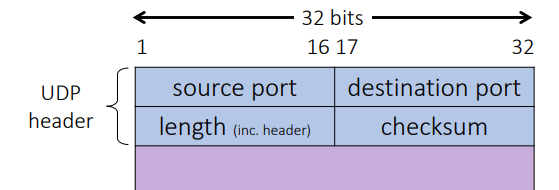
\includegraphics[width=0.9\linewidth]{UDP.png}
\end{center}

\section{Transmission Control Protocol}
\begin{itemize}
    \item Benefits:
    \begin{itemize}
        \item Connection-oriented, handshake must be established
        \item Reliable, in-order byte stream, segments have Maximum Segment Size (MSS) which does NOT include header
        \item Flow control: Sender cannot flood receiver
        \item Congestion control: Throttle sender if network is overloaded
        \item Guaranteed delivery
    \end{itemize}
    \begin{itemize}
        \item No guarantee on throughput
        \item More resources needed and increased delay
    \end{itemize}
    \item Sequence Number: Byte number of first byte of data in segment
    \item Acknowledgment Number: Sequence number of next byte of data expected, cumulative ACK
    \item TCP Timeout Value: Too short causes retransmissions, too long causes slow reaction to loss
    \begin{itemize}
        \item Estimating RTT: $RTT_E=(1-a) \cdot RTT_E + a \cdot RTT_S$, typically $a=1/8$, exponential weighted moving average
        \item Deviation of RTT: $RTT_{dev}=(1-b) \cdot RTT_{dev}+b \cdot |RTT_S-RTT_E|$, typically $b=1/4$
        \item Retransmission Time Out: $RTO = RTT_E+4\times RTT_{dev}$ using estimate and safety margin
    \end{itemize}
    \item Fast Retransmission: If 3 duplicate ACKs are received, resend segment immediately
    \item Connection Establishment: 3-way handshake
    \begin{itemize}
        \item Client sends TCP SYN and initial sequence number
        \item Server chooses initial sequence number, sends TCP SYN and ACK
        \item Client sends ACK
    \end{itemize}
    \item Half-Open Connections: Vulnerable to SYN Flooding or SYN/ACK flooding
    \item Closing Connection: Each side closes their own side of connection, by sending segments with FIN bit, after which they can no longer send data
    \item Flow Control: Receiver buffers data to application, and tells sender how much data it can send, sender can send 0-data segment to check when buffer empties
\end{itemize}
\begin{center}
    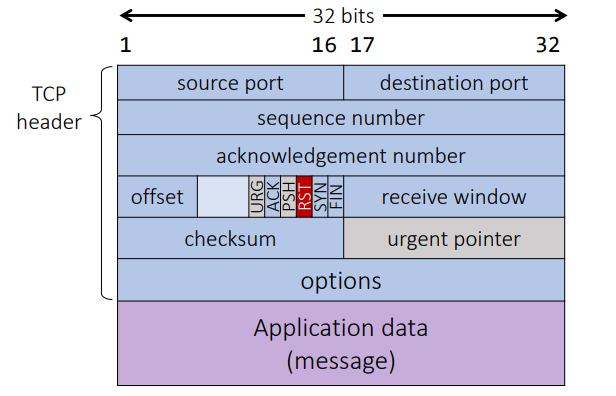
\includegraphics[width=0.9\linewidth]{TCP.png}
\end{center}

\section{Tutorial Content}
\subsection{Message Segmentation}
\begin{itemize}
    \item Without message segmentation, the whole packet must be retransmitted if there are bit errors that cannot be tolerated
    \item Without message segmentation, huge packets are sent into the network which routers have to accommodate for, and smaller packets have to queue behind
    \item However, packets must be put back in sequence at the destination
    \item Many smaller packets must also carry their own headers which causes some overhead
\end{itemize}
\subsection{Topology}
\begin{itemize}
    \item Minimum links: Simpler and cheaper, but has many points of failure that could crippler network, along with having longer paths between nodes
    \item Maximum links: More robust and faster travel, but is expensive
\end{itemize}
\subsection{DNS}
\begin{itemize}
    \item Suppose $n$ DNS servers are visited each with RTT of $D_{DNS}$
    \item Let $D_{Web}$ denote RTT between local host and server of each object
    \item For five objects and three DNS servers:
    \item Non-persistent HTTP with no parallel TCP connections: $3D_{DNS}+(5+1)\times 2 \times D_{Web}$
    \item Non-persistent HTTP with parallel TCP connections: $3D_{DNS}+2 \times D_{Web} + 2\times D_{Web}$, as the HTML file must be first fetched before which the 5 objects can be fetched in parallel
    \item Persistent HTTP with pipelining: $3D_{DNS}+2\times D_{Web}+D_{Web}$, as the HTML needs to be fetched first before each of the 5 objects can be fetched in parallel over the same connection 
    \item DNS Cache Poisoning: Rogue DNS records are introduced into DNS resolver's cache, causing name server to return an incorrect IP address and divert traffic to the attacker
\end{itemize}
\subsection{Sequence Numbers}
\begin{itemize}
    \item Large sequence numbers are used to prevent collisions
    \item TTL is specified in IP packet header to prevent packets from circulating
    \item Increases by number of bytes sent, not with segments sent
\end{itemize}

\end{multicols*}

\end{document}